The previous chapter introduced a probabilistic framework that can be used to design algorithms for robot localization and state estimation. The chapter concluded with the introduction of the Bayes filter, which is a fundamental algorithm for maintaining and updating a belief distribution (a probability distribution over possible states). While the Bayes filter is generally intractable to implement in practice, it lays a mathematical foundation for the development of algorithms that can exploit structure or other approximations to generate tractable approaches. One such example is the discrete Bayes filter, which assumes that the number of possible states is finite such that the belief distribution can be represented by simply storing the probability of each state individually. This type of distribution is referred to as \textit{non-parametric} since the belief distribution is not required to have a particular structure.

Alternatively, it is possible to develop tractable algorithms for probabilistic localization and state estimation by leveraging \textit{parametric} belief distributions. Parametric distributions are distributions that are fully specified by a fixed number of parameters, for example Gaussian distributions are defined by the mean and covariance parameters. These \textit{parametric filters} can generally be viewed as practical implementations of Bayes filter that exploit structure for efficiency, and include the Kalman filter family of algorithms.

\notessection{Parametric Filters}
Parametric filters\cite{ThrunBurgardEtAl2005} are a family of algorithms for robot localization and state estimation that model the robot's belief with parametric distributions. Therefore, as the robot's state evolves and new measurement information arrives, updating the belief distribution is accomplished by simply updating the parameters that define the distribution. This can lead to practically implementable algorithms since the number of parameters is generally not too large. For example, a Gaussian distribution in one dimension only requires the specification of two parameters: the mean and standard deviation. Yet with these two parameters a probability distribution is defined over an infinite number of values! This is an example of how parametric filters exploit structure for efficiency.

\subsection{Gaussian Distribution}
The Gaussian distribution (also referred to as a normal distribution) is likely the most commonly used parametric distribution in many disciplines, including robotics. The probability density function for a one-dimensional (univariate) Gaussian distribution is given by:
\begin{equation}
p(x) = \frac{1}{\sqrt{2\pi \sigma^2}} e^{-\frac{1}{2}\frac{(x-\mu)^2}{\sigma^2}},
\end{equation}
where the parameters are the mean $\mu$ and standard deviation $\sigma$ (the quantity $\sigma^2$ is referred to as the variance). A shorthand notation for saying that a random variable $X$ is distributed according to a Gaussian (normal) distribution is $X \sim \mathcal{N}(\mu,\sigma^2)$.
For the multi-dimensional case, the multivariate Gaussian distribution is defined by the probability density function:
\begin{equation}
p(\x) = \frac{1}{\sqrt{\text{det}(2\pi \bSigma)}} \text{exp}\big( -\frac{1}{2}(\x-\bmu)^\top  \bSigma^{-1} (\x-\bmu) \big),
\end{equation}
where $\x\in \R^n$ and the parameters are the mean $\bmu \in \R^n$ and the covariance matrix $\bSigma \in \R^{n \times n}$. Again, a shorthand to say a random variable $X$ is distributed according to the multivariate Gaussian distribution is $X \sim \mathcal{N}(\bmu,\bSigma)$. These distributions are represented graphically for the univariate and bivariate case in Figure \ref{fig:Gaussians}.
\begin{figure}[ht]
\centering
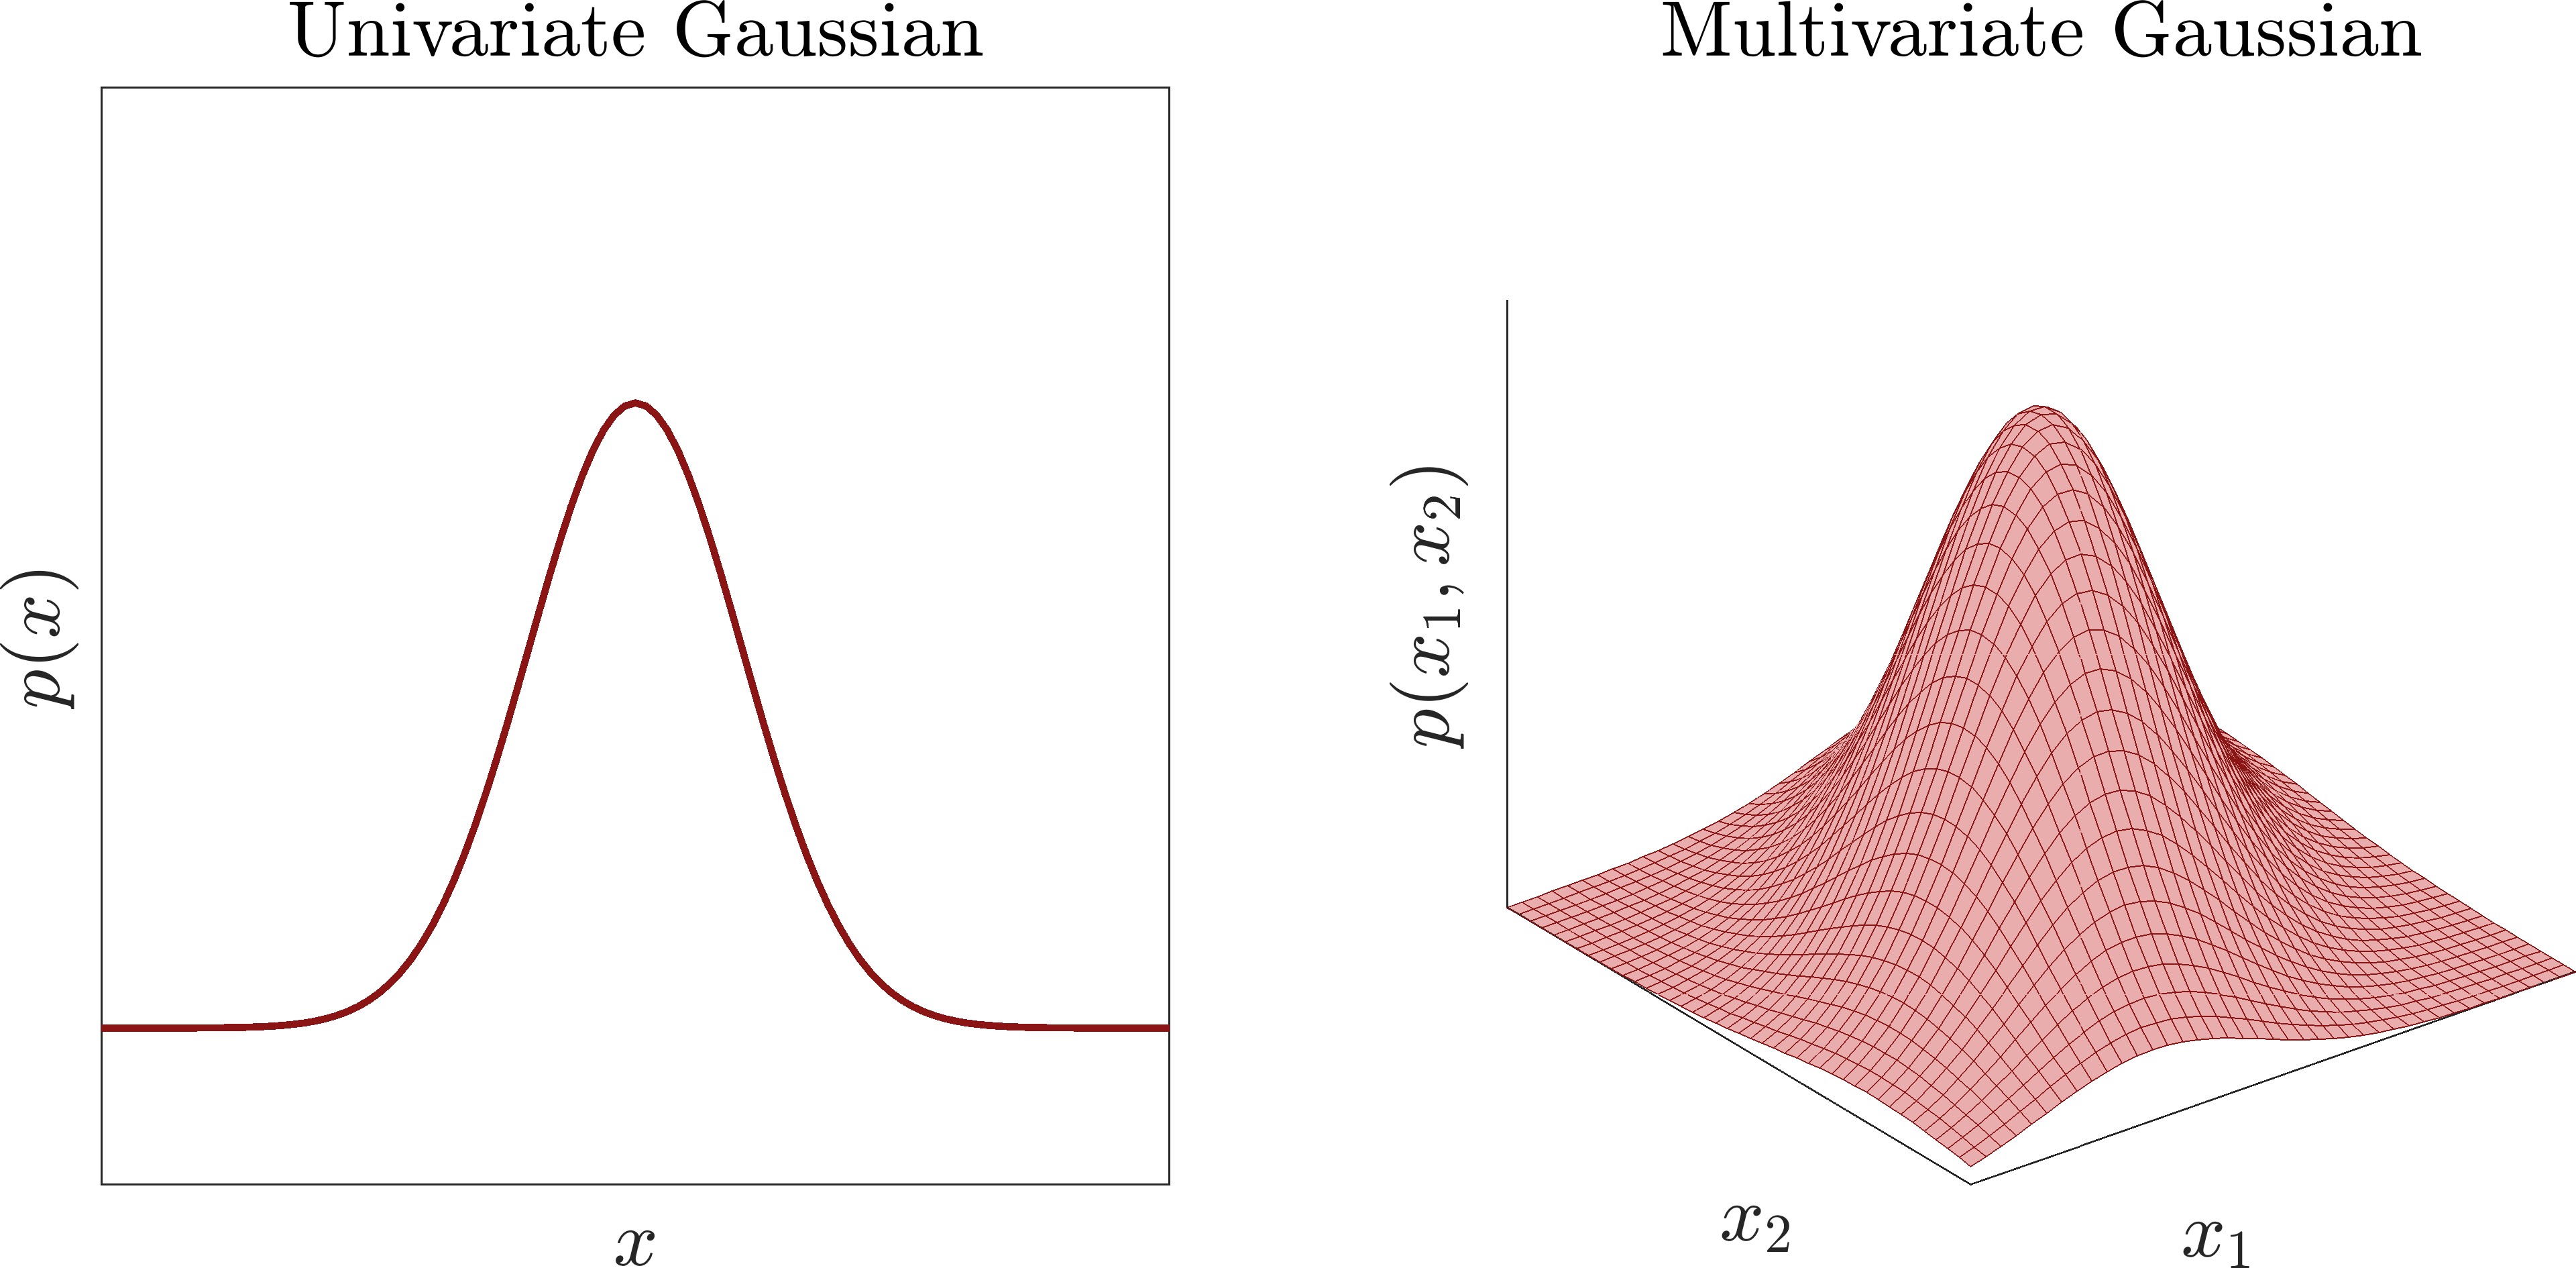
\includegraphics[width=.85\textwidth]{tex/figs/ch14_figs/gaussians.png}
\caption{Univariate and multivariate Gaussian distributions.}
\label{fig:Gaussians}
\end{figure}
These distributions exhibit several important properties which make them particularly attractive for algorithm development:
\begin{enumerate}
    \item The affine transformation of a Gaussian random variable is also a Gaussian random variable. In particular, suppose the random variable $X$ has a multivariate Gaussian distribution with mean $\bmu$ and covariance $\bSigma$. Then the random variable $Y$ resulting from an affine transformation:
    \begin{equation*}
        Y = AX + b,
    \end{equation*}
    also has a multivariate Gaussian distribution with expected value $A\bmu + b$ and covariance $A\bSigma A^\top $. In other words, if $X \sim \mathcal{N}(\bmu, \bSigma)$ then $Y \sim \mathcal{N}(A\bmu+b, A\bSigma A^\top )$.
    \item The sum of two independent Gaussian random variables is also a Gaussian random variable. In particular, suppose $X_1$ and $X_2$ have multivariate Gaussian distributions with means $\bmu_1$ and $\bmu_2$ and covariances $\bSigma_1$ and $\bSigma_2$. Then the random variable $Y$ given by the sum:
    \begin{equation*}
        Y = X_1 + X_2,
    \end{equation*}
    also has a multivariate Gaussian distribution with expected value $\bmu_1 + \bmu_2$ and covariance $\bSigma_1 + \bSigma_2$. In other words, if $X_1 \sim \mathcal{N}(\bmu_1, \bSigma_1)$ and $X_2 \sim \mathcal{N}(\bmu_2, \bSigma_2)$ then $Y \sim \mathcal{N}(\bmu_1 + \bmu_2, \bSigma_1 + \bSigma_2)$.
    \item The product of two Gaussian random variables is also a Gaussian random variable.
\end{enumerate}

\subsection{Kalman Filter}
The Kalman filter is an extremely well known algorithm for state estimation that leverages the Gaussian distribution for efficiency. Unlike the discrete Bayes filter from the previous chapter, this filter can be applied to problems with \textit{continuous} states.
In particular, a multivariate Gaussian distribution is used to parameterize the belief distribution over possible states, in other words the state $\x_t \sim \mathcal{N}(\bmu_t, \bSigma_t)$, and in long form this can be expressed as:
\begin{equation*}
bel(\x_t) = p(\x_t) = \frac{1}{\sqrt{\text{det}(2\pi \bSigma_t)}} \text{exp}\big( -\frac{1}{2}(\x_t-\bmu_t)^\top  \bSigma_t^{-1} (\x_t-\bmu_t) \big).
\end{equation*}

\subsubsection{Assumptions}
To ensure that the belief \textit{remains} Gaussian after the prediction and measurement update steps of the filtering algorithm, several additional assumptions are required.
First, it is assumed that the initial belief $bel(\x_0)$ is Gaussian with $\x_0 \sim \mathcal{N}(\bmu_0, \bSigma_0)$ and that the state transition model is linear and is given by:
\begin{equation} \label{eq:KFdynamics}
    \x_t = A_t \x_{t-1} + B_t \bu_t + \bm{\epsilon}_t,
\end{equation}
where $\x_{t-1}$ is the previous state, $\bu_t$ is the most recent control input, and $\bm{\epsilon}_{t}$ is an independent \textit{process noise} that is normally distributed with $\bm{\epsilon}_t \sim \mathcal{N}(\bm{0},\bm{R}_t)$.
Because of the properties of the Gaussian distribution presented earlier, this affine model preserves the Gaussian structure. In particular, the state transition model can be explicitly written as:
\begin{equation*}
p(\x_t \mid \x_{t-1}, \bu_t) = \frac{1}{\sqrt{\text{det}(2\pi \bm{R}_t)}} \text{exp}\big( -\frac{1}{2}(\x_t-A_t \x_{t-1} - B_t \bu_t)^\top  \bm{R}_t^{-1} (\x_t-A_t \x_{t-1} - B_t \bu_t) \big).
\end{equation*}
In other words, this can be expressed in shorthand as $\x_t \sim \mathcal{N}(A_t \x_{t-1} + B_t \bu_t, \bm{R}_t)$.

Second, the measurement model is also assumed to be linear, which again preserves the Gaussian structure:
\begin{equation} \label{eq:measure}
\z_t = C_t \x_t + \bm{\delta}_t,
\end{equation}
where $\bm{\delta}_t$ is an independent measurement noise that is normally distributed with $\mathcal{N}(\bm{0},\bm{Q}_t)$.
Again, this implies the measurement model can be expressed probabilistically as:
\begin{equation*}
p(\z_t \mid \x_t) = \frac{1}{\sqrt{\text{det}(2\pi \bm{Q}_t)}} \text{exp}\big( -\frac{1}{2}(\z_t-C_t\x_t)^\top  \bm{Q}_t^{-1} (\z_t-C_t\x_t) \big),
\end{equation*}
and in shorthand as $\z_t \sim \mathcal{N}(C_t \x_{t}, \bm{Q}_t)$.

To summarize, if the belief is modeled as a Gaussian distribution and the state transition and measurement models are both linear with Gaussian noise, then the Bayes filter updates can be applied and the belief will always remain Gaussian (i.e. the prediction and measurement correction steps will not warp or alter the \textit{structure} of the belief distribution)! This results in a very practically efficient algorithm since now only the parameters $\bmu$ and $\bSigma$ need to be updated by the algorithm.


\subsubsection{Algorithm}
The Kalman filter algorithm is a recursive Bayes filter whose prediction and measurement correction steps take on a special form due to the structure of the Gaussian belief distributions and the assumptions listed above.
In particular, the Kalman filter algorithm is given in Algorithm \ref{alg:KF}.

\begin{algorithm}[ht]
 \KwData{$\bmu_{t-1}, \bSigma_{t-1}, \bu_{t},\z_{t}$}
 \KwResult{$\bmu_t, \bSigma_t$}
 $\bar{\bmu}_t = A_t\bmu_{t-1}+B_t \bu_t$\\
 $\bar{\bSigma}_t = A_t\bSigma_{t-1} A_t^{T} + \bm{R}_t$\\
 $K_t = \bar{\bSigma}_{t}C_t^{T}(C_t\bar{\bSigma}_{t}C_t^{T}+\bm{Q}_t)^{-1}$\\
 $\bmu_t = \bar{\bmu}_t + K_t(\z_t-C_t\bar\bmu_{t})$\\
 $\bSigma_t = (I-K_tC_t )\bar{\bSigma}_t$\\
 \Return $\bmu_t, \bSigma_t$
 \caption{Kalman Filter Algorithm}
 \label{alg:KF}
\end{algorithm}
In this algorithm, the first two steps define the predicted mean $\bar{\bmu}_t$ and covariance $\bar{\bSigma}_t$, and the remaining steps perform the measurement correction. The matrix $K_t$ that is computed for the measurement correction is typically referred to as the \textit{Kalman gain}.

\subsubsection{Practical Considerations}
Due to the exploitation of the Gaussian distribution, the Kalman filter is a computationally efficient algorithm that can handle continuous state values. However, the consideration of Gaussian beliefs also restricts the flexibility of the probabilistic model. In particular, the belief is forced to be unimodal which may limit performance. Additionally, the assumption about the linearity of the state transition and measurement models may not be very accurate for some robots and certain sensors, which can make the Kalman filter not perform well for some robotics applications. 

\subsubsection{Derivation}
While it is possible to derive the Kalman filter algorithm by evaluating the Bayes filter updates from the previous chapter (i.e. computing the integral of $p(\x_t \mid \x_{t-1}, \bu_t) p(\x_{t-1}$, etc.), it is more intuitive to directly leverage the properties of Gaussians presented in the preceding section. First, from the prior belief distribution $bel(\x_{t-1}) \sim \mathcal{N}(\bmu_{t-1},\bSigma_{t-1})$ the predicted belief $\overline{bel}(\x_{t-1})$ can be computed by using the affine transformation property of Gaussian random variables and the sum of two independent Gaussian random variables property. Specifically, these properties can be applied to the assumed linear state transition model \eqref{eq:KFdynamics} to give:
\begin{equation*}
\begin{split}
\bar{\bmu}_t &= A_t \bmu_{t-1} + B_t\bar{\bu}_t + \bm{0}, \\
\end{split}
\end{equation*}
where the $\bm{0}$ is the mean of the independent noise $\bm{\epsilon}_t \sim \mathcal{N}(\bm{0},\bm{R}_t)$. The covariance properties can similarly be used to give:
\begin{equation*}
\begin{split}
\bar{\bSigma}_t &= A_t \bSigma_{t-1}A_t^\top  + \bm{R}_t. \\
\end{split}
\end{equation*}

For the measurement update it is possible to again use the properties of Gaussians to simplify the derivation of the Kalman filter measurement correction step. In particular, that the product of two Gaussians is also Gaussian. In fact, the product of the two Gaussians:
\begin{equation*}
\begin{split}
bel(x_t) = p(\z_t \mid \x_t)\overline{bel}(\x_t) &= \mathcal{N}(C_t\x_t,\bm{Q}_t) \mathcal{N}(\bar{\bmu}_{t},\bar{\bSigma}_{t}), \\
\end{split}
\end{equation*}
can be expressed as:
\begin{equation*}
\begin{split}
bel(x_t) = \eta\: \text{exp}\big(-\frac{1}2 J_t \big),
\end{split}
\end{equation*}
where $\eta$ is a normalization constant and:
\begin{equation*}
    J_t = (\z_t-C_t\x_t)^\top  \bm{Q}_t^{-1} (\z_t-C_t\x_t) + (\x_t-\bar{\bmu}_t)^\top  \bar{\bSigma}_t^{-1} (\x_t-\bar{\bmu}_t).
\end{equation*}
To determine the mean $\bmu_t$ and covariance $\bSigma_t$ of this new Gaussian, one simple approach is just take the first and second derivative of $J_t$ with respect to $\x_t$. The mean is found where the first derivative is zero, and the covariance is the (inverse) of the constant second derivative:
\begin{equation*}
\begin{split}
0 &= -C_t^\top  \bm{Q}_t^{-1}(\z_t - C_t \bmu_t) + \bar{\bSigma}_t^{-1}(\bmu_t - \bar{\bmu}_t), \\   
\bSigma_t^{-1} &= C_t^\top  \bm{Q}_t^{-1} C_t + \bar{\bSigma}_t^{-1}.
\end{split}
\end{equation*}
Through some algebraic manipulation the mean can be written in terms of the covariance $\bSigma_t$:
\begin{equation*}
\begin{split}
\bmu_t &= \bar{\bmu}_t + \bSigma_t C_t^\top  \bm{Q}_t^{-1}(\z_t - C_t \bar{\bmu}_t), \\
\end{split}
\end{equation*}
and of course the covariance can be written as:
\begin{equation*}
\begin{split}
\bSigma_t &= (C_t^\top  \bm{Q}_t^{-1} C_t + \bar{\bSigma}_t^{-1})^{-1}.
\end{split}
\end{equation*}
While it is technically possible to stop here, this is not quite the form of the Kalman filter equations. In particular a few more algebraic steps are needed, based on the matrix inversion lemma result:
\begin{equation*}
(C_t^\top  \bm{Q}_t^{-1} C_t + \bar{\bSigma}_t^{-1})^{-1} = \bar{\bSigma}_t - \bar{\bSigma}_tC_t^\top (C_t\bar{\bSigma}_tC_t^\top  + \bm{Q}_t)^{-1}C_t\bar{\bSigma}_t.
\end{equation*}
By choosing to define the Kalman gain as $K_t = \bar{\bSigma}_{t}C_t^{T}(C_t\bar{\bSigma}_{t}C_t^{T}+\bm{Q}_t)^{-1}$ it can be seen that the covariance can be expressed as:
\begin{equation*}
\begin{split}
\bSigma_t &= \bar{\bSigma}_t - K_tC_t\bar{\bSigma}_t,
\end{split}
\end{equation*}
Through some additional algebra, the expression for the mean can also be expressed in terms of the Kalman gain and simplified to its final form:
\begin{equation*}
\bmu_t = \bar{\bmu}_t + K_t(\z_t-C_t\bar\bmu_{t}).
\end{equation*}
For more details on the algebraic steps see Thrun et al.\cite{ThrunBurgardEtAl2005}.


%%%%%%%%%%%%%%%%%%%%%%%%%%%%%%%%%%%%%%%%%%%%%%%%%%
\subsection{Extended Kalman Filter (EKF)}
The extended Kalman filter (EKF) is a modified version of the Kalman filter that revisits the assumption of linearity for the state transition and measurement models. This extension still exploits the Gaussian distribution to represent the belief in a computationally efficient parametric way, but by generalizing to more complex models the EKF can be applied to a wider variety of robotics state estimation and localization problems. In particular, the EKF considers general nonlinear state transition and measurement models defined as:
\begin{equation}
\begin{split}
\x_t &= g(\bu_t, \x_{t-1}) + \bm{\epsilon}_{t}, \\
\z_t &= h(\x_t) + \bm{\delta}_{t},
\end{split}
\end{equation}
where again $\bm{\epsilon}_{t}\sim \mathcal{N}(\bm{0},\bm{R}_t)$ and $\bm{\delta}_{t}\sim \mathcal{N}(\bm{0},\bm{Q}_t)$ are normally distributed noise terms.

The EKF handles these nonlinear functions by taking advantage of their first order Taylor series expansions (which are linear functions, similar to those used in the Kalman filter). In particular the Taylor series expansion of the state transition model $g$ is performed about the \textit{most likely state} from the current belief distribution, which is the expected value $\bmu_{t-1}$:
\begin{equation*}
\begin{split}
g(\bu_t, \x_{t-1}) &\approx g(\bu_t, \bmu_{t-1}) + G_t (\x_{t-1}-\bmu_{t-1}), \\
\end{split}
\end{equation*}
where $G_t = \nabla_{\x} g(\bu_t, \bmu_{t-1})$ is the Jacobian of $g$ evaluated at $\bmu_{t-1}$. From this linear approximation the state transition model can be expressed as:
\begin{equation*}
p(\x_t \mid \x_{t-1}, \bu_t) = \frac{1}{\sqrt{\text{det}(2\pi \bm{R}_t)}} \text{exp}\big( -\frac{1}{2}\Delta \x_t^\top  \bm{R}_t^{-1} \Delta \x_t \big),
\end{equation*}
where
\begin{equation*}
\Delta \x_t = \x_t-g(\bu_t, \bmu_{t-1}) - G_t (\x_{t-1}-\bmu_{t-1}).
\end{equation*}
From this result, the linear predictions that are used in the Kalman filter algorithm can be replaced by the nonlinear generalizations:
\begin{equation*}
\begin{split}
\bar{\bmu}_t &= g(\bu_t,\bmu_{t-1}), \\
\bar{\bSigma}_t &= G_t\bSigma_{t-1} G_t^{T} + \bm{R}_t.
\end{split}
\end{equation*}
As can be seen the prediction of the new mean is simply an evaluation of the nonlinear function $g$, and the updated covariance is very similar to the Kalman filter but leverages the Jacobian $G_t$.

A very similar procedure is used for the measurement corrections. The measurement model is also Taylor series expanded to yield (this time about the \textit{predicted} point $\bar{\bmu}_t$):
\begin{equation*}
\begin{split}
h(\x_t) \approx h(\bar{\bmu}_t) + H_t (\x_{t}-\bar{\bmu}_{t}), \\
\end{split}
\end{equation*}
where $H_t = \nabla_{\x} h(\bar{\bmu}_{t})$ is the Jacobian of $h$ evaluated at $\bar{\bmu}_{t}$. The measurement model can then be expressed using this approximation as:
\begin{equation*}
p(\z_t \mid \x_t) = \frac{1}{\sqrt{\text{det}(2\pi \bm{Q}_t)}} \text{exp}\big( -\frac{1}{2}\Delta \z_t^\top  \bm{Q}_t^{-1} \Delta \z_t \big),
\end{equation*}
where $\Delta \z_t = \z_t-h(\bar{\bmu}_t) - H_t (\x_{t}-\bar{\bmu}_{t})$. From this result the measurement correction in the EKF can be shown to be similar to the Kalman filter, but where the Jacobians $H_t$ are used:
\begin{equation*}
\begin{split}
\bmu_t &= \bar{\bmu}_t + K_t(\z_t - h(\bar{\bmu}_{t})), \\
\bSigma_t &= (I - K_t H_t)\bar{\bSigma}_t,
\end{split}
\end{equation*}
where the Kalman gain is $K_t = \bar{\bSigma}_{t}H_t^{T}(H_t\bar{\bSigma}_{t}H_t^{T}+\bm{Q}_t)^{-1}$.

\subsubsection{Algorithm}
The extended Kalman filter algorithm is quite similar to the Kalman filter algorithm outlined in Algorithm \ref{alg:KF}. In particular the main differences are that the updates use the nonlinear functions and their Jacobians rather than assuming strictly linear models. The EKF algorithm is outlined in Algorithm \ref{alg:ekf}.
\begin{algorithm}[ht]
 \KwData{$\bmu_{t-1}, \bSigma_{t-1}, \bu_{t},\z_{t}$}
 \KwResult{$\bmu_t, \bSigma_t$}
 $\bar{\bmu}_t = g(\bu_t,\bmu_{t-1})$\\
 $\bar{\bSigma}_t = G_t\bSigma_{t-1} G_t^{T} + \bm{R}_t$\\
 $K_t = \bar{\bSigma}_{t}H_t^{T}(H_t\bar{\bSigma}_{t}H_t^{T}+\bm{Q}_t)^{-1}$\\
 $\bmu_t = \bar{\bmu}_t + K_t(\z_t - h(\bar{\bmu}_{t}))$\\
 $\bSigma_t = (I - K_t H_t)\bar{\bSigma}_t$\\
 \Return $\bmu_t, \bSigma_t$
 \caption{Extended Kalman Filter Algorithm}
 \label{alg:ekf}
\end{algorithm}

\subsubsection{Practical Considerations}
The extended Kalman filter can provide more accurate results than the Kalman filter in many applications due to its ability to consider more general nonlinear models. However, the approximation of the nonlinear models by a Taylor series expansion can lead to the filter to diverge if the approximation is not accurate enough.
Additionally, the EKF still suffers from the same unimodal modeling assumption as the Kalman filter since the beliefs are still represented by a single Gaussian distribution.

\subsection{Unscented Kalman Filter}
The unscented Kalman filter (UKF) is another variation of the Kalman filter (still uses Gaussian distribution to parameterize the belief). This filter is also similar to the EKF in that it can handle nonlinear state transition and measurement models. However, this filter improves upon the EKF by not relying on Taylor series expansions, which can cause filter divergence due to approximation errors. 
This is accomplished by representing the Gaussian through a set of \textit{sigma-points} that are transformed through the nonlinear functions. Once each sigma-point has been updated, a new Gaussian distribution is computed to represent the updated belief.

\subsection{Exercises}
\subsubsection{EKF Localization}
Complete \textit{Problem 1: EKF Localization} located in the online repository:

\vspace{\baselineskip}

\url{https://github.com/PrinciplesofRobotAutonomy/AA274A_HW4},

\vspace{\baselineskip}

where you will implement an EKF for robot localization based on linear feature extraction and a map of known features.